\documentclass{sig-alternate-10pt}

\newcommand{\ttt}{\texttt}

\usepackage{graphicx}
\usepackage{changepage}
\usepackage{lipsum}

\title{FLASH\\Fast Linux Advanced Scheduler Hardware}
\author{
	Mark Aligbe \\
	    \email{ma2799@columbia.edu}
	\and
    Chae Jubb \\
        \email{ecj2122@columbia.edu}
}
\date{7 April 2015}

\begin{document}
\maketitle

\begin{abstract}
\lipsum[1]
\end{abstract}


\section{Introduction}
\lipsum[1]

\section{Scheduling in the Kernel}
% Mark
\lipsum[1]

\section{FLASH Architecture}
The FLASH hardware unit is built with ease of replacement of the usual
software implementation in mind.  The major addition we add over a standard
scheduler is the ability for the scheduler itself to raise an interrupt to
indicate a tick. Figure~\ref{fig:arch_overview} gives an overview of the
system architecture.

\begin{figure}
	\begin{center}
		%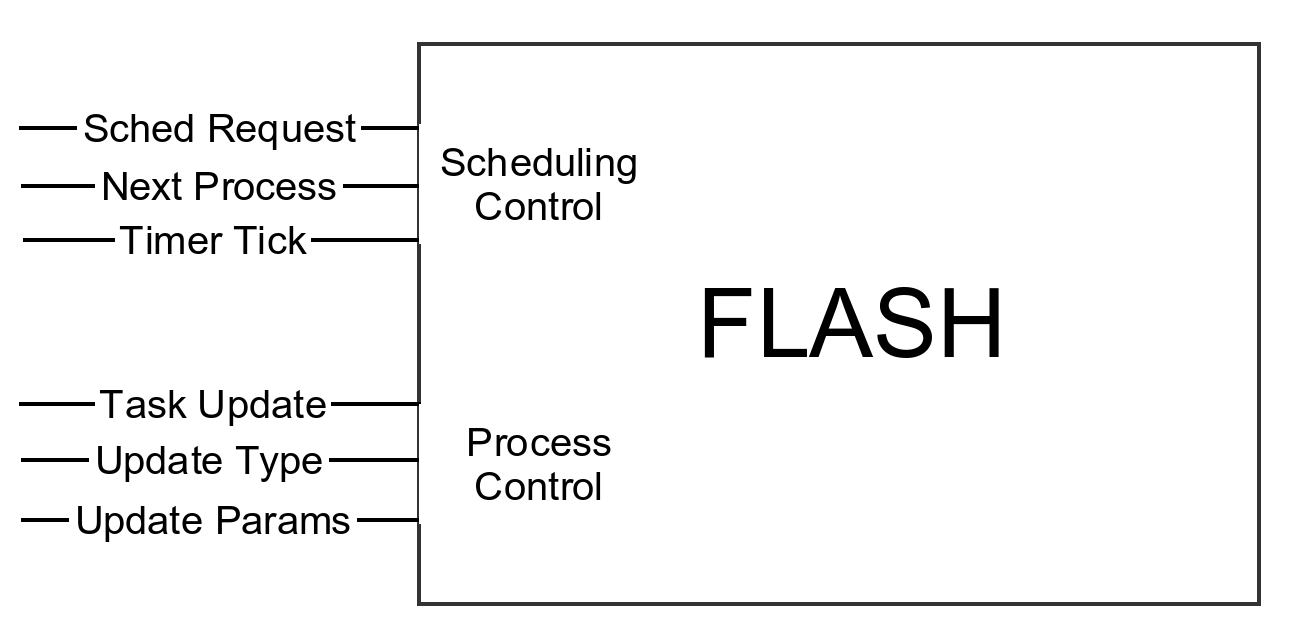
\includegraphics[width=0.65\textwidth]{fig/flash-diagram.png}
		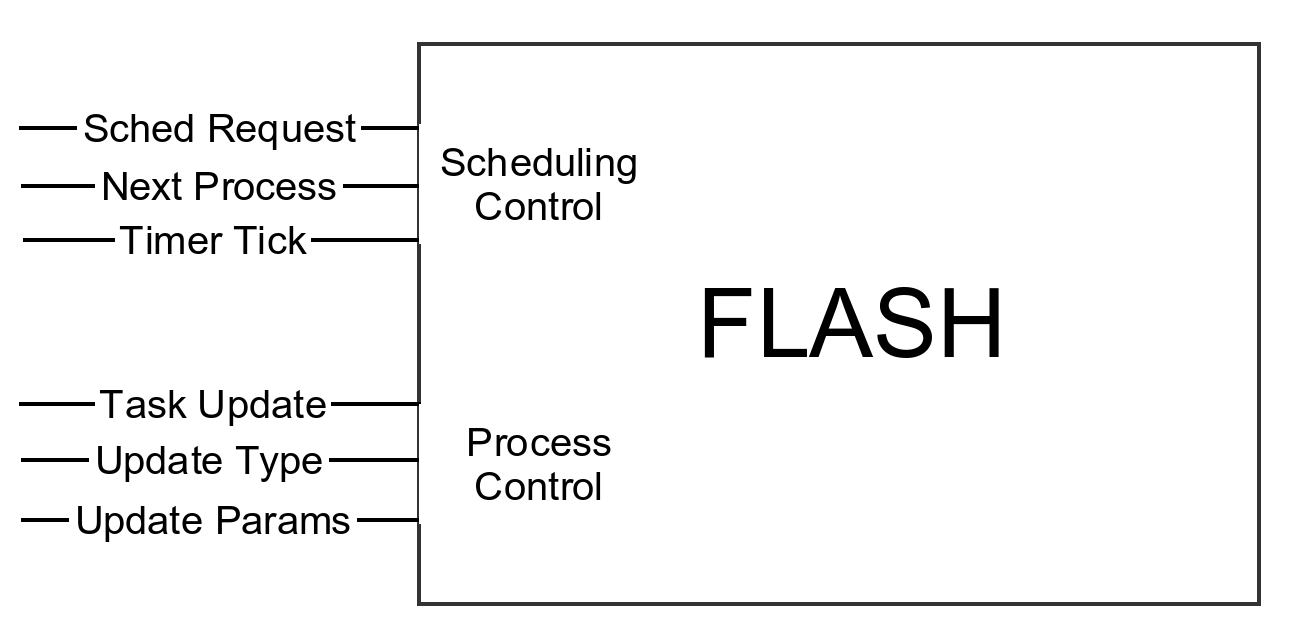
\includegraphics[width=0.9\linewidth]{fig/flash-diagram.png}
		\caption{
			FLASH System Architecture: Interface.  Note the distinction between
			the \emph{Process Control} and \emph{Scheduling Control} Interfaces.
		}
		\label{fig:arch_overview}
	\end{center}
\end{figure}

We now describe in more detail both the interface and
internal implementation of the scheduling unit.

\subsection{FLASH Interface}
At its most basic, the hardware interface is given by two major segments:
\emph{scheduling control} and \emph{process control}.  Together these two
segments allow processes to be scheduled based on an up-to-date accounting
of process status, kept via the process control interface.  The scheduling
controller interface sends timer tick interrupts and serves incoming
requests for new processes to run.

\subsubsection{Process Control Interface}
Let us first focus deeply on this process control interface.  It is here
that FLASH is given information to hold the proper state of all running
processes.  Currently, we store process id (PID), priority, and state
triples as passed through the interface using a standard four-phase
handshake.

\paragraph{Consistency} A major hurdle with offloading scheduling decisions
to a dedicated piece of hardware is ensuring consistency between the data
structures maintained by the software kernel (again, here Linux) and the
hardware unit.

We cannot completely offload the data about processes to hardware most
obviously because of sheer size of objects like the \ttt{task\_struct} as
well as their high use by modules other than the scheduler.  We must,
though, retain some structure in FLASH memory so that it may make even the
most basic scheduling decisions.

For this reason, we expect each update in process priority or state to be
communicated to FLASH so it may continue making accurate scheduling
decisions.

\subsubsection{Scheduling Control Interface}
In addition to the process control interface, FLASH provides a scheduling
control interface, responsible for providing the software with tasks to be
run.  We can further subdivide this interface into two subparts: scheduling
requests and timer ticks.  Making replacement of software more
straightforward, these subparts directly correspond to the two main modes of
tasks switching in the Linux Kernel.

\paragraph{Scheduling Requests}
Often a running process will want to do something (such as disk I/O) that
requires yielding the processor.  When this occurs, the Linux kernel will
call \texttt{schedule()}.  We modify this schedule function to interact with
our scheduling control interface, more specifically the portion dealing with
scheduling requests.

A scheduling request will be received using a standard four-phase handshake.
At this point, using methods explained in Section~\ref{sec:FLASH_impl}, the
next task to be run is selected and returned to the software.

\paragraph{Timer Tick}
FLASH also provides functionality to raise an interrupt via a timer tick.
For simplicity and fully encapsulating scheduling logic, we export the
generation of the timer tick to this hardware unit.  At a specified time
interval, FLASH will raise a timer interrupt and provide the software with
the next task to be run.

\subsection{FLASH Implementation}
\label{sec:FLASH_impl}
FLASH aims to implement a CFS scheduling algorithm\footnote{The current
implementation is a prioritized round robin algorithm.}, allowing
transparent replacement of the current software implementation.  Internally,
we have two front-end modules, each corresponding to a segment of the
interface (process control and scheduling control). Those front-end modules
connect to back-end modules which regulate and control access to the backing
internal data structures.  We see this internal implementation architecture
described in Figure~\ref{fig:impl_overview}.

\begin{figure*}
	\begin{center}
		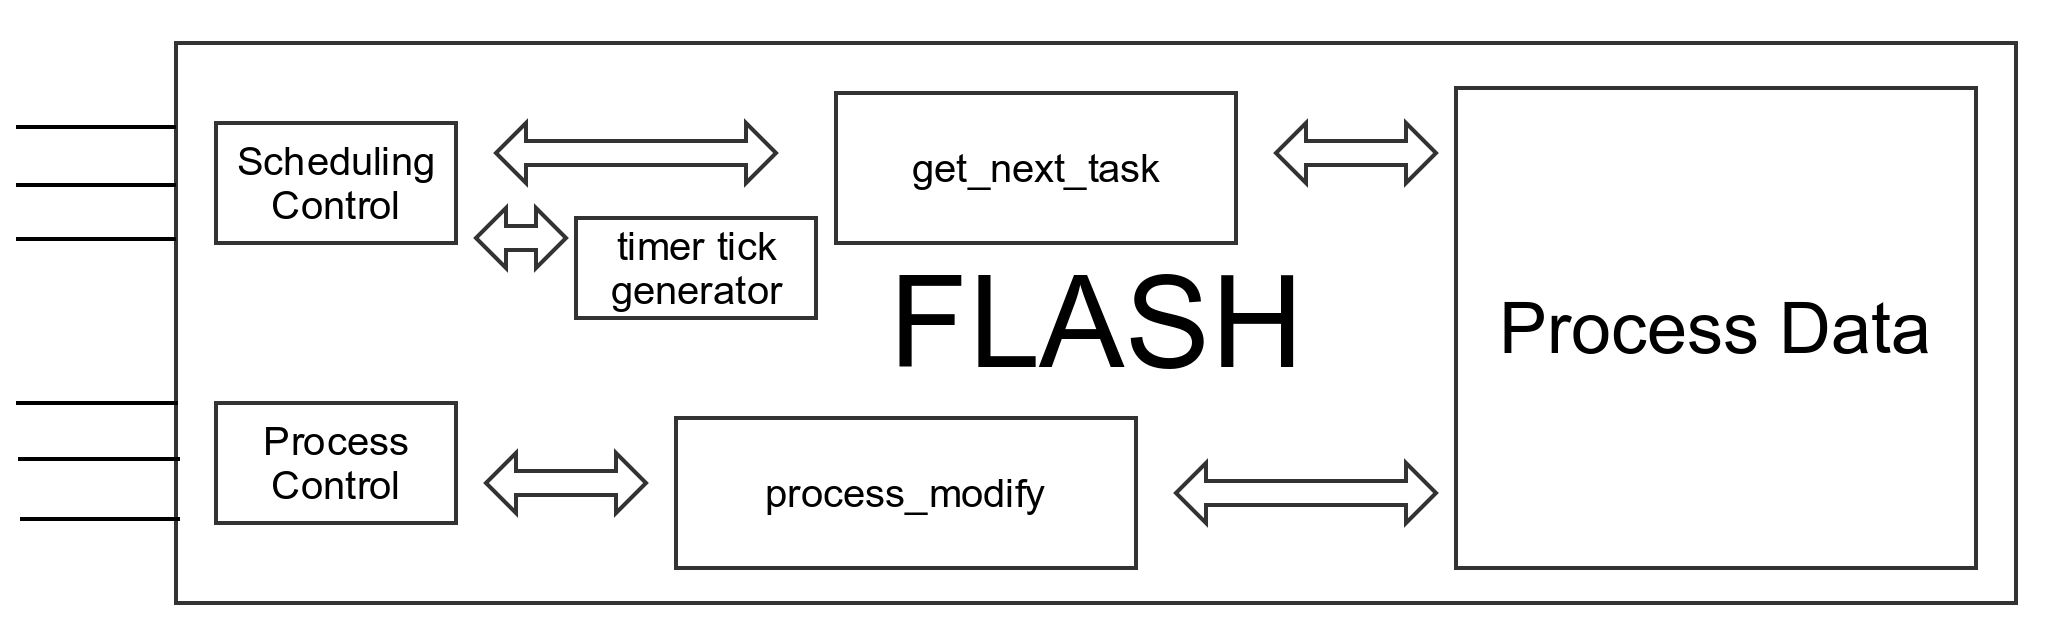
\includegraphics[width=0.9\textwidth]{fig/flash-impl.png}
		%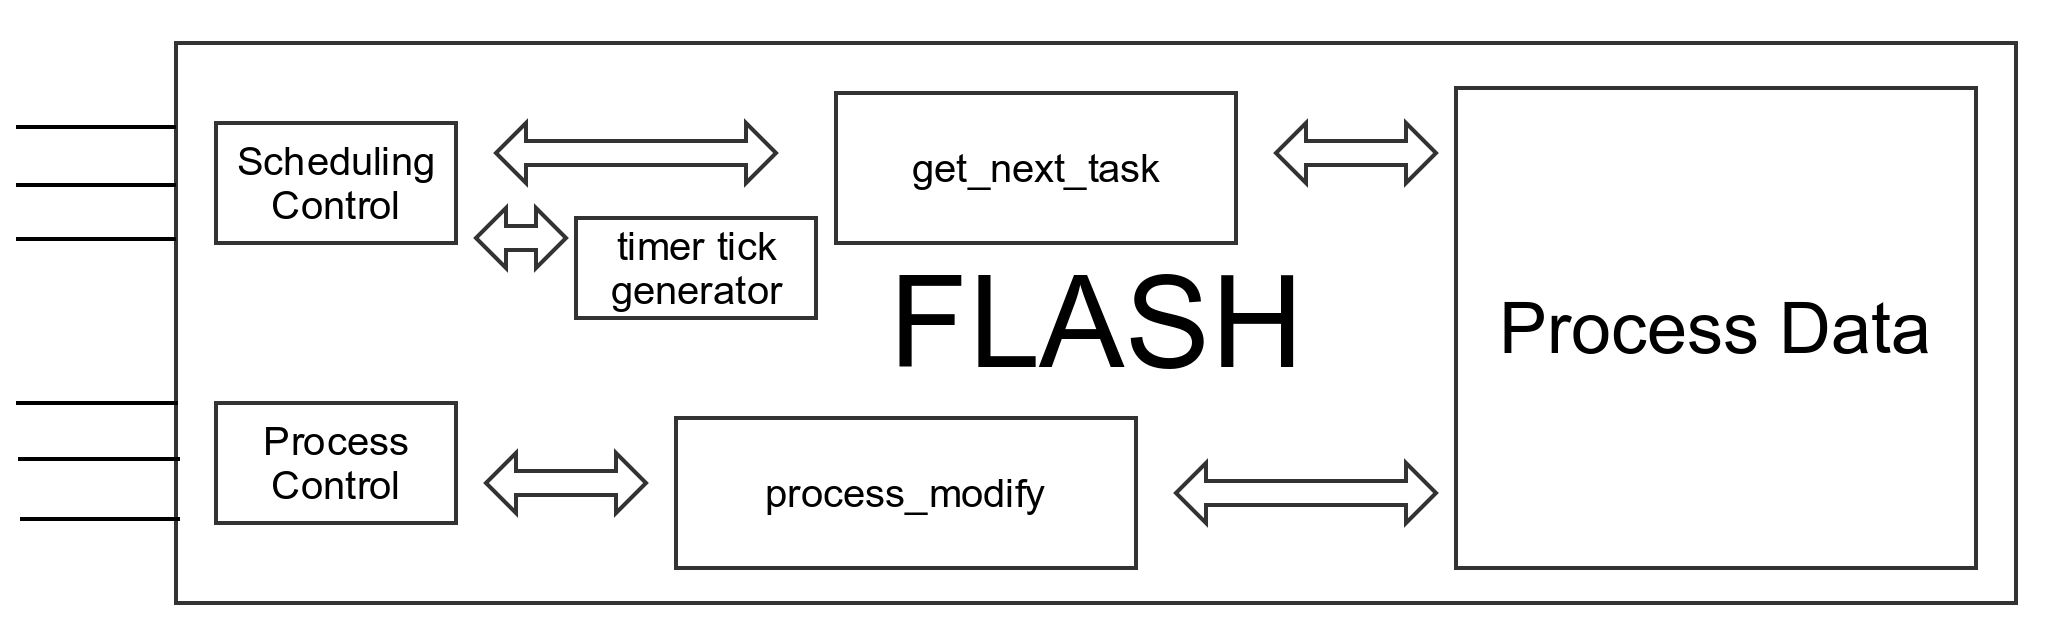
\includegraphics[width=0.9\linewidth]{fig/flash-impl.png}
		\caption{
			FLASH System Architecture: Implementation.  Notice the division
			between the front-end, back-end, and process data modules.  This
			allows tightly regulated access to backing process data store.
		}
		\label{fig:impl_overview}
	\end{center}
\end{figure*}

\subsubsection{Front-End Modules}
As mentioned above, we have a front-end module for each segment of the
interface.  Each of these modules is quite simple.  The module corresponding
to the scheduling control interface has two jobs: responding to scheduling requests
as well as passing on timer ticks generated by a different internal module.
Both of these require querying for the next task to be run.

The second front-end module corresponds to the process control interface.
It will simply communicate through the incoming request and update the
backing store of process state.

\subsubsection{Back-End Modules}
The FLASH back-end modules serve to regulate access to the backing data
store.  This is done via two modules: a reading module and a writing module.
The process control datapath is connected through the writing module as this
interface is used to modify the state of processes.

Additionally, we have a simple reading module connected to the scheduling
control interface.  This regulates reads to the backing data store in order
to determine the next process that ought to be run.

\subsubsection{Storing Process State}
The current FLASH implementation is a basic version of CFS.  We do not use
the same type of implementation as the Linux kernel because implementing
red-black trees in hardware would be prohibitively complex.  Instead we use
a series of simple queues that are sorted with priority in mind.

The FLASH scheduling algorithm, like CFS, will keep record of the runtime of
the process as well as a \emph{virtual runtime}.  This virtual runtime is a
weighted accounting of the actual runtime based on priority of the process.
Scheduling decisions are made based on the virtual runtime, as in CFS.

\paragraph{On Red-Black trees}
While using a red-black tree would allow the implementation to be
algorithmically faster, actual runtime in software will likely be higher
than iterating through a simple queue implemented in hardware.  Firstly,
hardware will simply be faster than software as it is more easily
parallelizable.  The hardware can parallelize comparisons in logarithmic
time, whereas an iteration in software will take linear time.

Secondly, traversing the red-black tree in software will not have ideal cache
performance. Switching to a self-contained hardware module will not have any
cache considerations because that hardware unit will have a single
monolithic memory.

\paragraph{What do we store?}
In addition to storing the PID, priority, and state, we also have a few
fields used to store internal state necessary to keep the CFS implementation
completely fair.  These fields most importantly include a notion of virtual
runtime.  Other fields are for bookkeeping reasons.

\subsection{Summary}
Together the interface and implementation of FLASH provide an easily
integrable scheduling module.  The kernel will interface with the hardware
unit in the same way that the software scheduler does.  Additionally, FLASH
implements the current default Linux scheduler CFS.

\section{Evaluation}
% Mark
\lipsum[1]

\section{Integration}
% Chae then Mark
FLASH has been developed using SystemC and High Level Synthesis (HLS)
techniques.  This allows the engineer to work at the algorithmic level of
abstraction.  Not only prototyping but also verification can complete at a
quicker pace at the system level.  Architectural tradeoffs can be fully
examined and explored at a quicker pace than with traditional RTL
development.  More potential designs can be analyzed, and a Pareto curve can
be generated.  Using that information, the most suitable design can be
chosen as a tradeoff between (generally) area and speed.

% more Mark stuff here


\section{Related Works}
% Chae
One of the major bottlenecks to server-class performance in interactive
desktop environments is that of the context switch and in particular
scheduling.  FLASH attempts to provide a hardware module which serves as the
scheduler for the Linux Kernel.  We replace the CFS from the kernel with our
own implementation in accordance with the major principles of the Completely
Fair Scheduler\cite{wong2008cfs}.

Previous hardware scheduling units focus completely on embedded systems with
a fixed number of tasks\cite{nakano1995hardware, morton2004hardware,
nacul2007hardware, kuacharoen2003configurable, park2008hardware}.  The major
novel challenge in escalating to a desktop Linux is handling the dynamic,
unbounded (from a realistic hardware perspective) number of tasks.


\section{Conclusion}
\lipsum[1]

\nocite{*}
{
	\bibliographystyle{abbrv}
	\bibliography{ref}
}

\end{document}
